
\chapter{模板使用指引}

\section{导言}

\LaTeX 的上手可能相较 Word 麻烦一些,但也没那么复杂。跟随本章给出的使用指引,应当能在较短的时间内编写并编译一些基础文档,加上稍许耐心,一天时间内应该便可将写好的文字套入到该模板中得到格式完好的毕业论文。当然,在熟悉了 \LaTeX 后,更应该直接使用 \LaTeX 进行毕业论文的撰写。:)

\section{环境配置}

\subsection{安装 \LaTeX}

下载 \LaTeX 发行版 \textbf{TexLive 2019} 并安装\footnote{如果有旧的 \LaTeX 软件,请先卸载}。可以从\href{http://mirror.ctan.org/systems/texlive/Images/}{这里}下载安装包 (\texttt{texlive2019.iso})。由于小文件众多,安装时间会较长 (比如 1 小时以上),请耐心等待安装完成。

\subsection{安装 TeXstudio}

实际上,使用纯文本编辑器 (比如 \texttt{NotePad++, Sublime Text, VS Code} 等) 就可以编写 \LaTeX 文档。但专业的面向 \LaTeX 的编辑器可以极大地减少新手入门的难度,比如会给出命令提示、可以很方便地配置编译命令、有更加友好的错误提示等。

本文推荐新手可采用多平台且开源的 TeXstudio 作为编辑软件。可从\href{https://github.com/texstudio-org/texstudio/releases/download/2.12.22/texstudio-2.12.22-win-qt5.exe}{这里 (2.12.22 版本)} 下载并安装 Texstudio。

安装完毕后,在软件主界面的菜单中,依次选择 `\texttt{选项 -> 设置 TeXstudio -> 构建 -> 默认编译器}',将其调整为 \texttt{XeLaTeX} 后,点击保存即可。

\section{编译本文档}

使用 TeXstudio 打开本模板根目录下的 \texttt{thesis.tex} 文件。点击图~\ref{fig:build} 中的绿色按钮即可对当前的 \texttt{.tex} 文档进行编译。

\begin{figure}[htb]
    \centering
    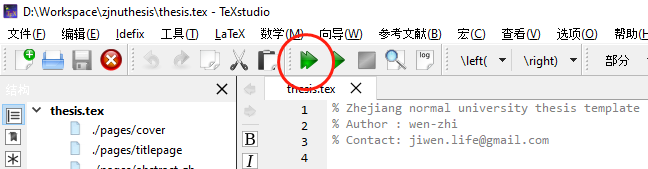
\includegraphics[width=\linewidth]{2-1-build}
    \caption{\label{fig:build} 编译按钮}
\end{figure}

静待编译完成后,即可得到该文档的 PDF 版本。至此,如果运行正常,则说明环境几乎配置完毕,已经迈过了使用 \LaTeX 的最大门槛,黎明就要来了。

\section{完善编译命令}

尽管上节中已经通过编译得到了最终的主文档,但可能存在超链接点击没反应 (比如点击目录中的项目无法进行跳转)、参考文献无法显示(比如这儿\cite{lecun2015deep}和这儿\cite{krizhevsky_imagenet_2012})等问题。这是因为仅一次编译无法得到 \texttt{.tex} 文档的所有信息。以参考文献为例,首先要经 \texttt{Biber} 编译文档得到参考文献的辅助文件后,然后再次运行 \texttt{XeLaTeX} 才能将参考文献信息嵌入到最终的文档中。

简而言之,需要得到完好的文档 (参考文献正常、超链接正常等) 需要经过多次的编译。编译顺序一般为 \texttt{XeLaTeX + Biber + XeLaTeX + XeLaTeX}。可通过设置 TeXstudio 提供的编译选项自定义多次编译命令,无需手动执行每次编译。

具体操作如下:

1) 依次打开 `\texttt{选项 -> 设置 TeXstudio -> 构建}',点击「用户命令」中的「添加」,再点击扳手图标

2) 首先删掉右侧的 \texttt{<Unknown>} (如果有),然后再从左侧依次将 \texttt{XeLaTeX, Biber, XeLaTeX, XeLaTeX, XeLaTeX} 添加到右侧,最后保存即可

\textbf{设置完毕后,可通过 `\texttt{工具 -> 用户}' 执行自定义的编译命令。}此时应能得到最终完好的文档\footnote{注意,不同于本文档,其超链接并没有使用彩色标记},注意观察上述参考文献的角标已经正常、超链接也均可访问。至此,环境配置彻底完毕,黎明已经到来。

需要注意的是,这种多次编译需要耗费较长的时间。因此如果暂不在乎参考文献的角标是否正常、超链接是否正常等,只需要查看文档的整体效果是否正常,可以仅执行一次 \texttt{XeLaTeX} 即可 (即点击一下图~\ref{fig:build} 的绿色按钮即可)。

\section{论文写作}

\subsection{导言}

环境配置完毕、完成第一次编译后,就基本迈过了使用 \LaTeX 的最大门槛,真正地进入「只关心内容」的状态,开始领会 \LaTeX 的独特魅力并\textbf{可能}会为之着迷。

本章将按照论文的顺序依次介绍各部分如何编辑完成。当读完本章时,应能对本模板的使用有一个基本的认识。

\subsection{个人信息}

打开主文档 \texttt{thesis.tex},填写姓名、学号、论文标题等信息,直接在原有的位置按照给出的示范进行填写。\textbf{不要引入额外的空行},严格遵循格式要求,\textbf{不要自己发挥}。

\subsection{封面}

由模板自动生成,无需使用者操心。:)

\subsection{扉页}

由模板自动生成,无需使用者操心。:)

\subsection{中文摘要}

打开 \texttt{pages} 文件夹下的 \texttt{abstract-zh.tex},输入中文摘要与关键词,然后保存。

\subsection{英文摘要}

打开 \texttt{pages} 文件夹下的 \texttt{abstract-en.tex},输入英文摘要与关键词,然后保存。

\subsection{正文}

打开 \texttt{body} 文件夹,分别对每个章节进行编辑。可按照相同的文件名模式自行添加新的章节,当然,同时也要在主文档 \texttt{thesis.tex} 中引入新的章节。

由于直接解释代码含义比较繁冗,且不直观,所以可直接对相应源码进行观察,自行体会其用法,接受起来也会非常轻松。比如,可打开本文所对应的 \texttt{chapter-1.tex, chapter-2.tex},并与本文档进行对比观察,即可知道如何进行章节的编写。这些写法都非常简单,自解释性足够强。

除了文字之外,文档中常见的元素还有图片、表格、公式等。相应的用法已经有足够多的优秀教程可供参考,用法不会太复杂,克服畏难情绪,稍稍坚持一会儿即可知道用法。

接下来,本节将对常见的文档元素 (图片、表格、公式等) 分别进行简单的介绍。同样,可以打开相应的源码部分,与实际的文档进行对照观察,这里先简单地认识一下这些元素的用法,打个照面。真正用到的时候可即时翻阅\href{http://mirrors.ctan.org/info/lshort/chinese/lshort-zh-cn.pdf}{《一份(不太)简短的 \LaTeXe 介绍》}的相关章节查阅用法,随查随用。

\subsubsection{图片}

首先将需要用到的所有图片均放于 \texttt{figures} 目录下,支持 \texttt{pdf, eps, png, jpg, bmp} 等格式。

图~\ref{fig:build}已经给出了一个单张图片的示例。可以观察其源代码,感受其用法。接下来给出一个多子图的示范,如图~\ref{fig:subfig} 所示。源代码中 \texttt{2-2-a, 2-2-b} 为相应的图片名,可以省略图片的后缀。\verb|\caption| 给出的则是题注。\verb|\label| 则用于给图片加标签,然后通过 \verb|\ref{标签名}| 进行引用。

\begin{figure}[htb]
    \centering
    \begin{subfigure}[b]{.4\linewidth}
        \centering
        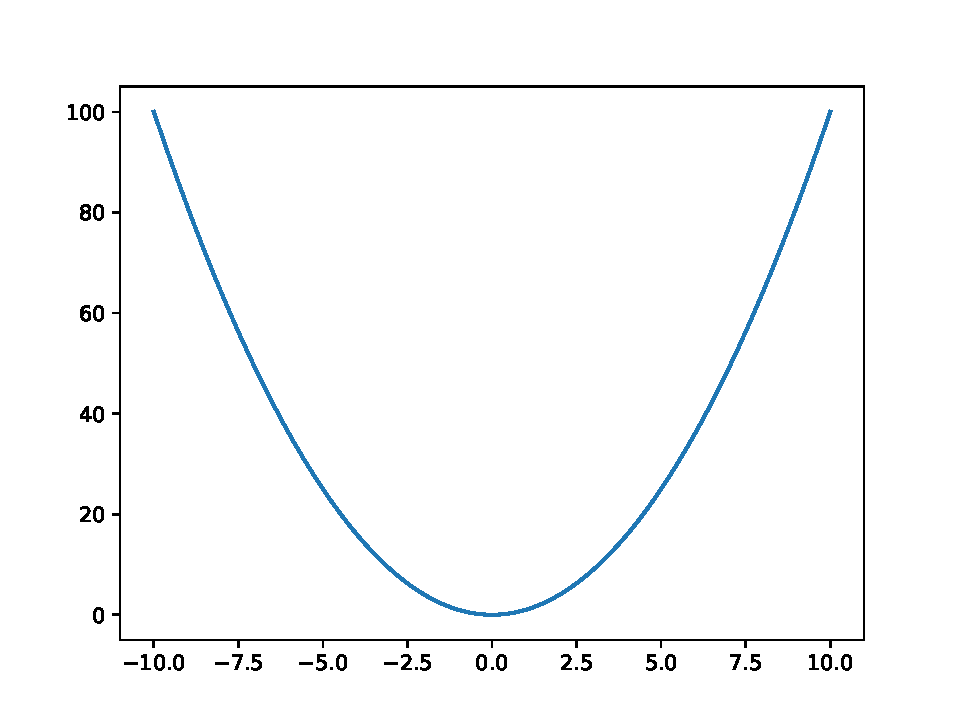
\includegraphics[width=\linewidth]{2-2-a}
        \caption{}
    \end{subfigure}
    ~%
    \begin{subfigure}[b]{.4\linewidth}
        \centering
        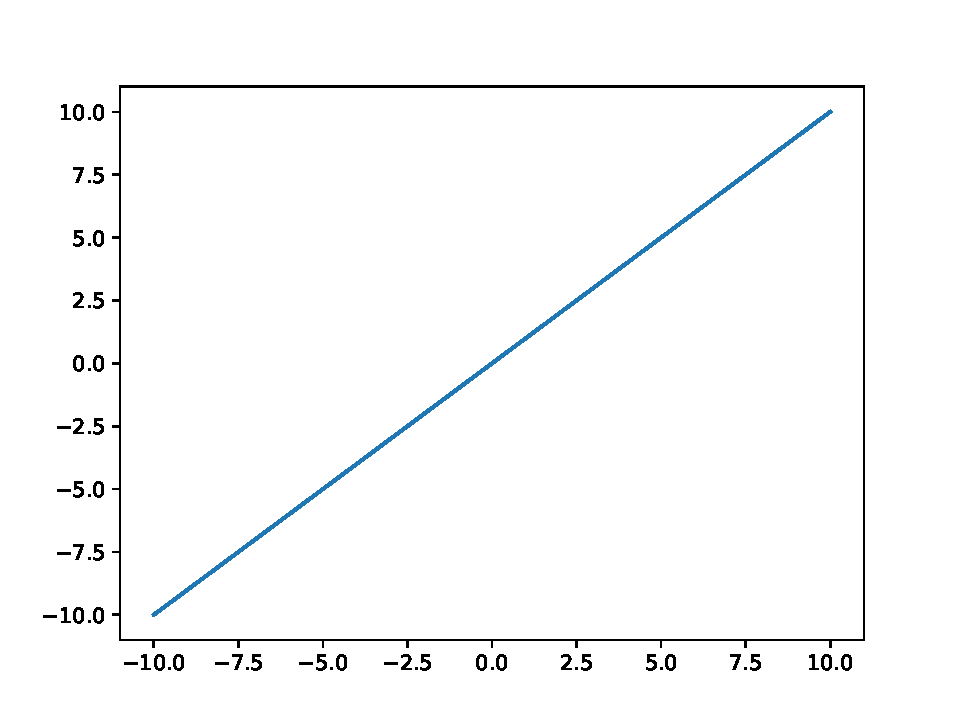
\includegraphics[width=\linewidth]{2-2-b}
        \caption{}
    \end{subfigure}
    \caption{\label{fig:subfig} 多子图示例}
\end{figure}

\subsubsection{表格}

表~\ref{table:decimal-to-binary} 给出了一个可变长度的表格示范。

\begin{table}[htb]
    \centering
    \caption{\label{table:decimal-to-binary}}
    \begin{tabularx}{.5\linewidth}{c X<{\centering\arraybackslash}}
        \hline
        decimal & binary \\
        \hline
        1 & 1 \\
        2 & 10 \\
        3 & 11 \\
        4 & 100 \\
        5 & 101 \\
        \hline
    \end{tabularx}
\end{table}

\subsubsection{公式}

将公式放入 \verb|equation| 环境内,即可被自动编号,同样也可以加标签,方便引用。既可以使用 \LaTeX 原生的 \verb|\ref| 进行引用,比如式~\ref{eq:example}。也可以使用 \verb|\eqref| 进行引用,比如式~\eqref{eq:example}。其差距在于,后者自动加上了一个括号。学校的规范里对选择何种样式没有要求,可依据自己的审美倾向选择喜欢的方式。

\begin{equation}
\label{eq:example}
a^2 + b^2 = c^2
\end{equation}

此外,模板预定义了部分常用但 \LaTeX 本身并未包含的命令,以更方便地书写向量、矩阵等,具体可见表~\ref{table:math}。

\begin{table}[htb]
    \centering
    \caption{\label{table:math} 模型预定义的一些数学命令}
    \begin{tabularx}{.5\linewidth}{c X<{\centering\arraybackslash}}
        \hline
        命令 & 效果 \\
        \hline
        \verb|\vec| & $\vec{x}, \vec{y}$ \\
        \verb|\mat| & $\mat{X}, \mat{y}$ \\
        \verb|\norm| & $\norm{x}, \norm{y}$ \\
        \verb|\argmax| & $\argmax_{x}\mathcal{L}(x)$ \\
        \verb|\argmin| & $\argmax_{x}\mathcal{L}(x)$ \\
        \hline
    \end{tabularx}
\end{table}

\subsubsection{算法}

算法的使用如算法~\ref{alg:euclid} 所示。具体的细节可在用到时翻阅 \verb|algorithmcx| 宏包的\href{http://mirrors.ctan.org/macros/latex/contrib/algorithmicx/algorithmicx.pdf}{文档}。

\begin{algorithm}
    \caption{\label{alg:euclid} 辗转相除法}
    \begin{algorithmic}[1]
    \Procedure{Euclid}{$a,b$}
    \State $r\gets a\bmod b$
    \While{$r\not=0$}
    \State $a\gets b$
    \State $b\gets r$
    \State $r\gets a\bmod b$
    \EndWhile\label{euclidendwhile}
    \State \textbf{return} $b$
    \EndProcedure
    \end{algorithmic}
\end{algorithm}

\subsection{参考文献}

当需要引用一个文献时,首先通过学术搜索引擎或通过文献管理软件导出该文献的 BibTeX 信息,然后将其复制到 \texttt{bib} 文件下的 \texttt{ref.bib} 文件中。

\begin{figure}[H]
    \centering
    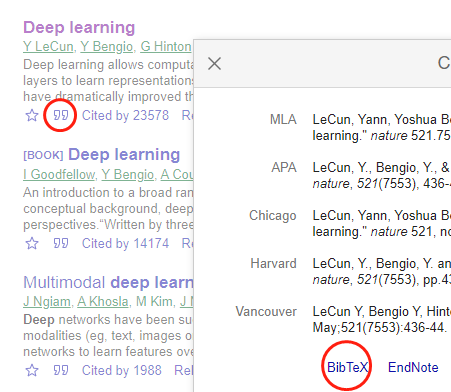
\includegraphics[width=0.7\linewidth]{2-3-ref}
    \caption{\label{fig:ref} 找到文献的 BibTeX 信息}
\end{figure}

例如,通过谷歌学术找到献的 BibTeX 信息 (如图~\ref{fig:ref} 所示) ,将其复制到 \texttt{ref.bib} 中后,即可通过 \verb|\cite{lecun2015deep}| 进行引用,比如\cite{lecun2015deep}。其中 \texttt{lecun2015deep} 为该文献的标签,是其 BibTeX 信息的第一行中所给出的信息。

而参考文献一章则由模板自动生成,无需使用操心。

\subsection{研究成果}

打开 \texttt{pages} 文件夹下的 \texttt{cv},填入自己的研究成果即可。

\subsection{致谢}

打开 \texttt{pages} 文件夹下的 \texttt{thanksto},填入致谢内容即可。

\subsection{诚信承诺书}

无需任何操作。

\subsection{独创性声明与授权声明}

无需任何操作。
